\section{Introduction}

\frame{
  \frametitle{Part of}
  \begin{figure}
    \includegraphics[width=0.8\textwidth]{figures/madelogo}
  \end{figure}
  Workpackage 8: Hyperflexible Automation
  %\pnote{My project was carried out as a part of MADE: Manufacturing Academy of Denmark. MADE is collaboration between various academic and industrial partners whose aim is to improve Denmark's domestic manufacturing capabilities. I was a part of MADEs WP8 entitled hyperflexible automation, however MADE itself deals will all aspects of manufacturing from supply chain management to quality assurance. But enough about that, let us get into todays topics.}
  \pnote{Domestic manufacturing. WP8 specifically. Many others: supply chain and QA}
}
\frame{
  \frametitle{3D Vision}
  \begin{minipage}[t]{0.48\linewidth}
    \begin{itemize}
      \item Use readily available 3D sensors.
      \item Solve problems.
      \item Both industrial and academical.
    \end{itemize}
  \end{minipage}
  \begin{minipage}[t]{0.48\linewidth}
    \begin{figure}
      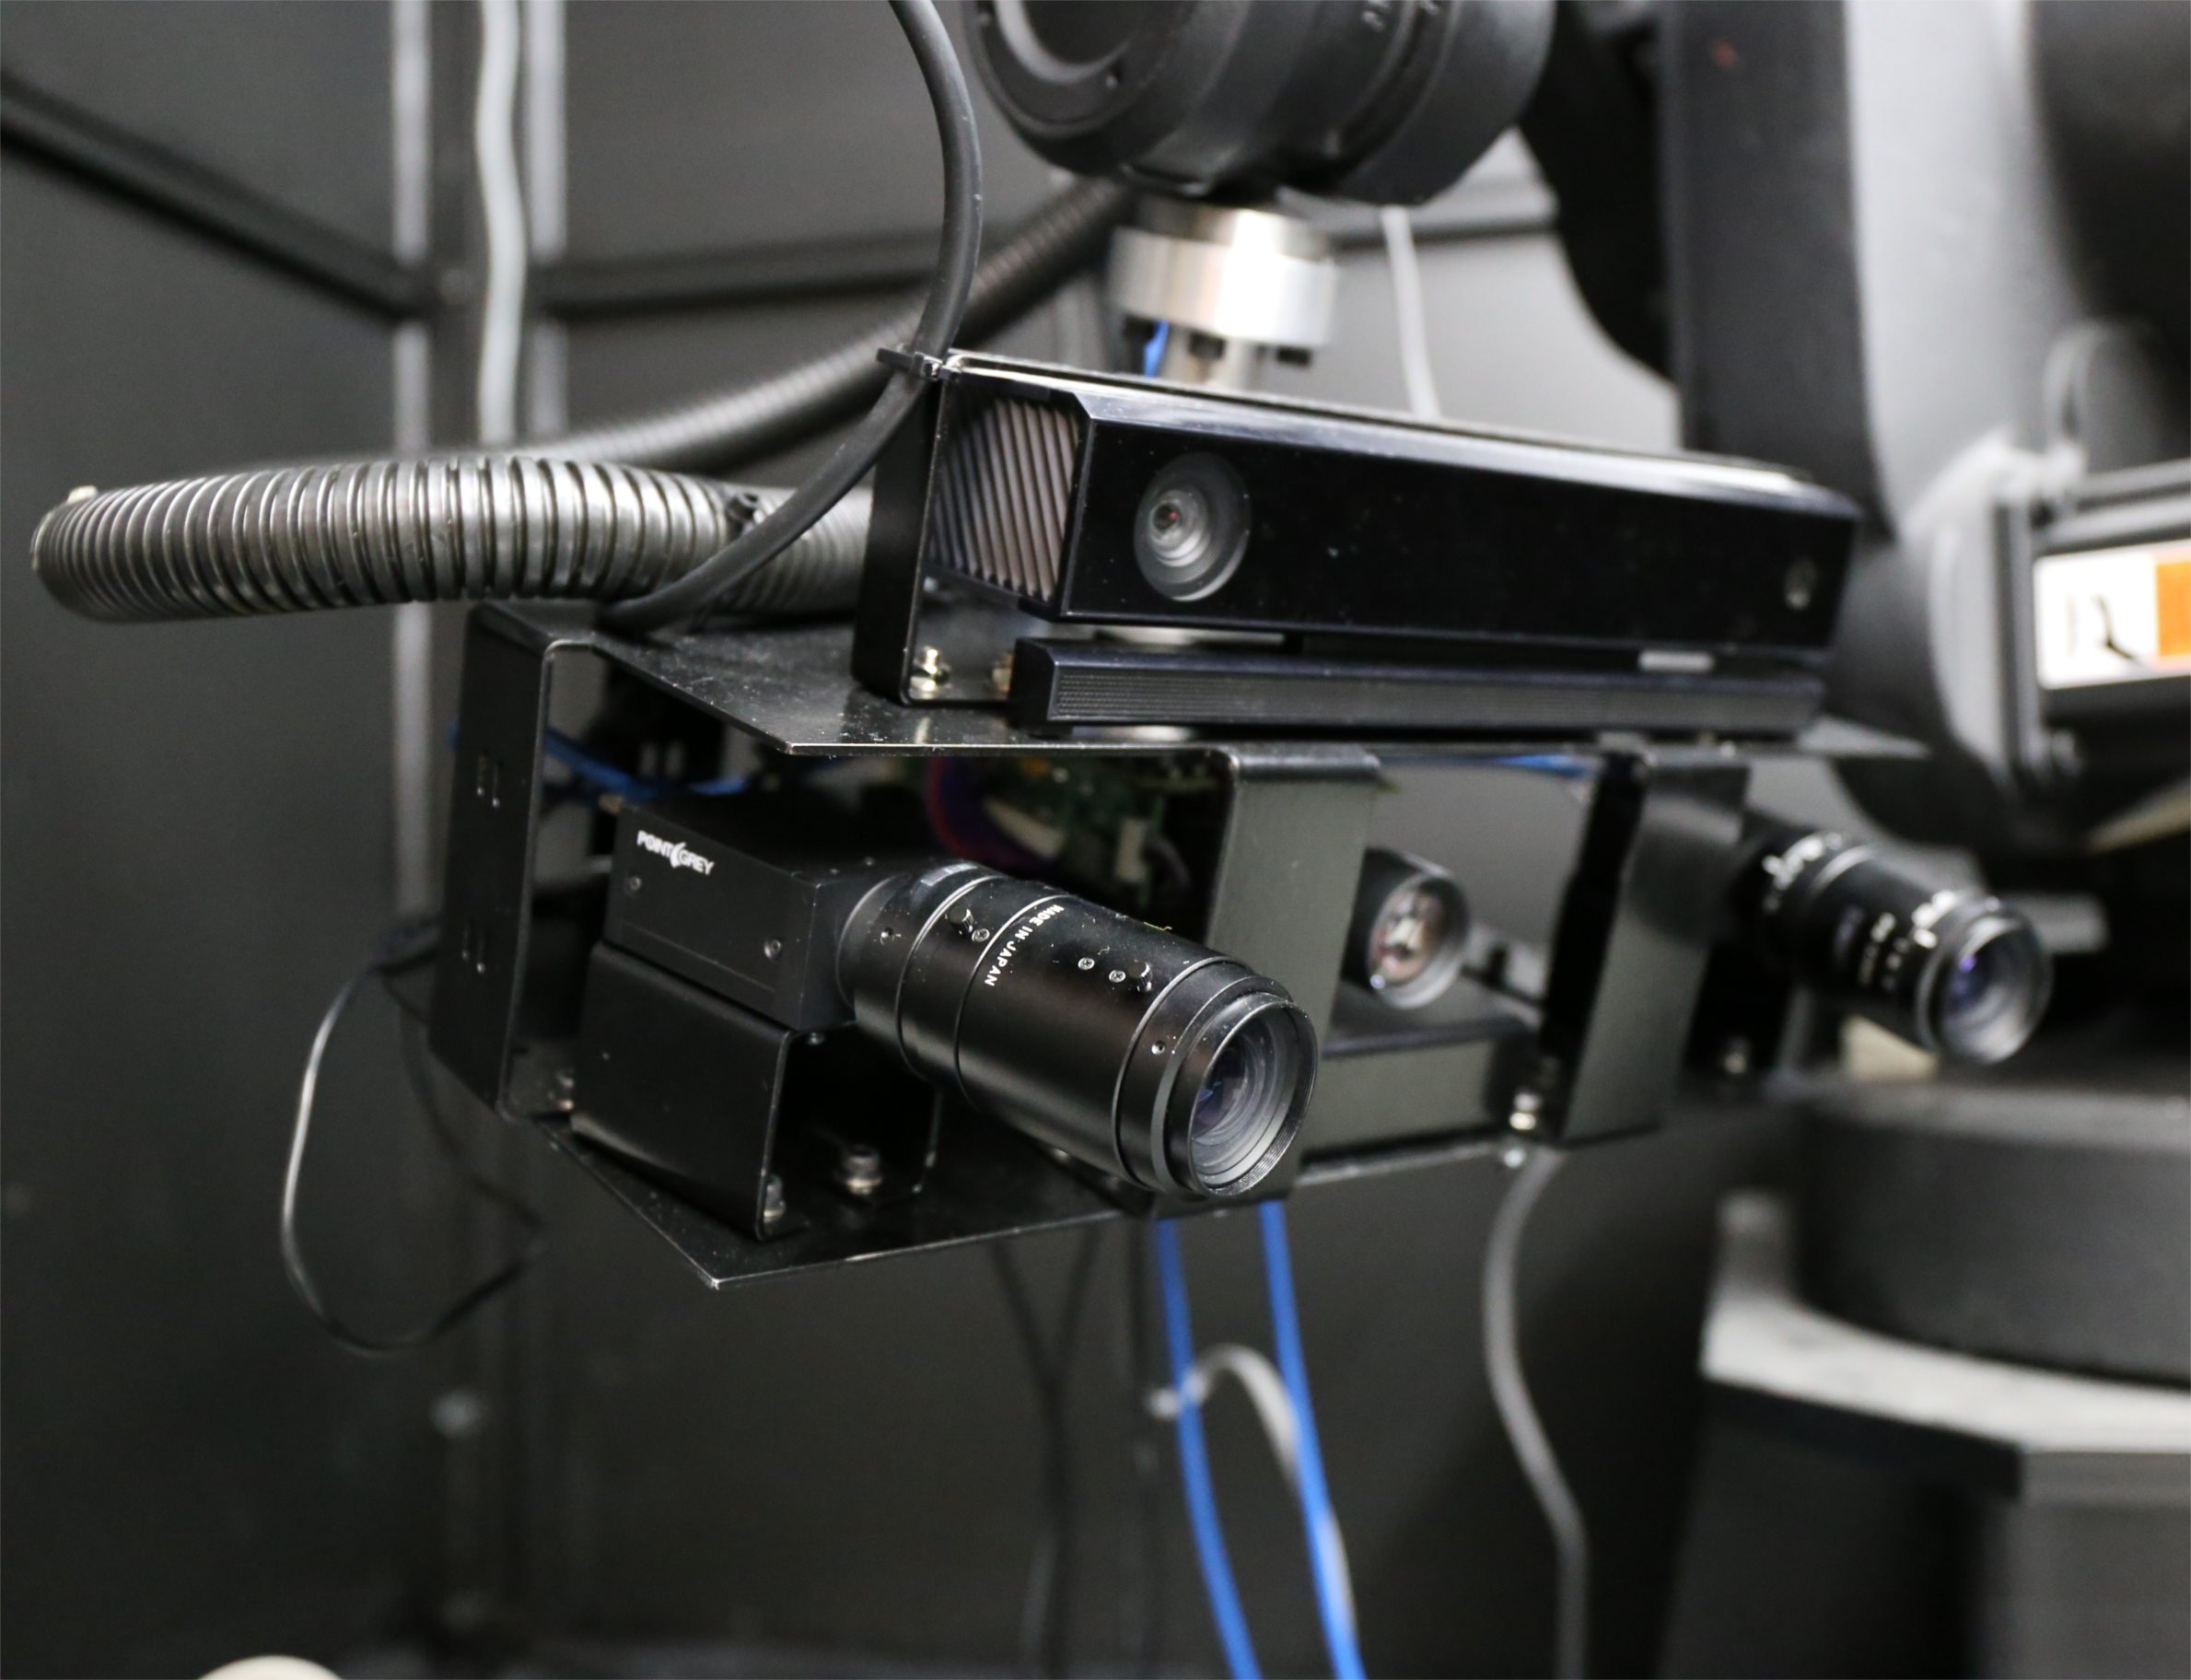
\includegraphics[width=1.0\linewidth]{figures/nrsfm_scanner}
    \end{figure}
  \end{minipage}
  \pnote{Recent advances. Widely vailable. Kinect or build yourself}
  %\pnote{The central theme of my thesis is 3D vision, that is technogoly that acquires 3D geometry from 2D image data. Advances in recent years has made this class of technology readily available to all. You can either buy one commercially (kinect V1) or simply put one together yourself provided that you have a couple of cameras and/or a projector. So the movitional problem behind my work was simply to use this technology to solve various problems of industrial and academical nature.}
}

\begin{comment}
\frame{
  \frametitle{Commercial 3D Sensors}
  \begin{figure}
    \includegraphics[width=0.35\linewidth]{figures/kinect}
    \hspace{2cm}
    \includegraphics[width=0.35\linewidth]{figures/gom}
  \end{figure}
  \begin{figure}
    \includegraphics[width=0.35\linewidth]{figures/bumblebee}
    \hspace{2cm}
    \includegraphics[width=0.35\linewidth]{figures/3df_zephyr_3_photogrammetry_statue}
  \end{figure}
}

\frame{
  \frametitle{3D Vision Application}
  \begin{figure}[t]
    \includegraphics[width=0.47\linewidth]{figures/selfdriving}
    \hfill
    \includegraphics[width=0.47\linewidth]{figures/baxter}
  \end{figure}
}

\frame{
  \frametitle{Real-world application can be surprisingly tricky...}
  \begin{figure}
    \centering
    \includegraphics[height=0.65\textheight]{figures/icecam}
    \hfill
    \includegraphics[height=0.65\textheight]{figures/failed2}
  \end{figure}
}
\end{comment}

\frame{
  \frametitle{Todays Topics}
  \tableofcontents
  \pnote{Exemplified. Mention structured light.}
}
